

%%%%%%%%%%%%%%%%%%%%%%%%%%%%%%%%%%%%%%%%%%%%%%%%%%%%%%%%%%%%%%%%%%%%%%%%%%%%%%
\section{Run 105038 : regular mode }

\subsection{Time distribution and occupancy}
In run 105038, the length of the event window was reduced to 25 us,
the rate of the FPGA internal pulsers was kept at 60 khZ. 

Similar to Section \ref{over}, Figure \ref{fig:4} shows the distributions
of the number of hits in two channels, one from the 
first and another one - from the second FPGA. 
In this readout configuration, the expected number of pulses in a given channel
within the event window is one or two, and the total number of pulses is always below 255.

\begin{figure}[H]
  \hspace{-0.5in}
  \begin{tikzpicture}
    \node[anchor=south west,inner sep=0] at (0,0.) {
      % \node[shift={(0 cm,0.cm)},inner sep=0,rotate={90}] at (0,0) {}
      % \makebox[\textwidth][c] {
      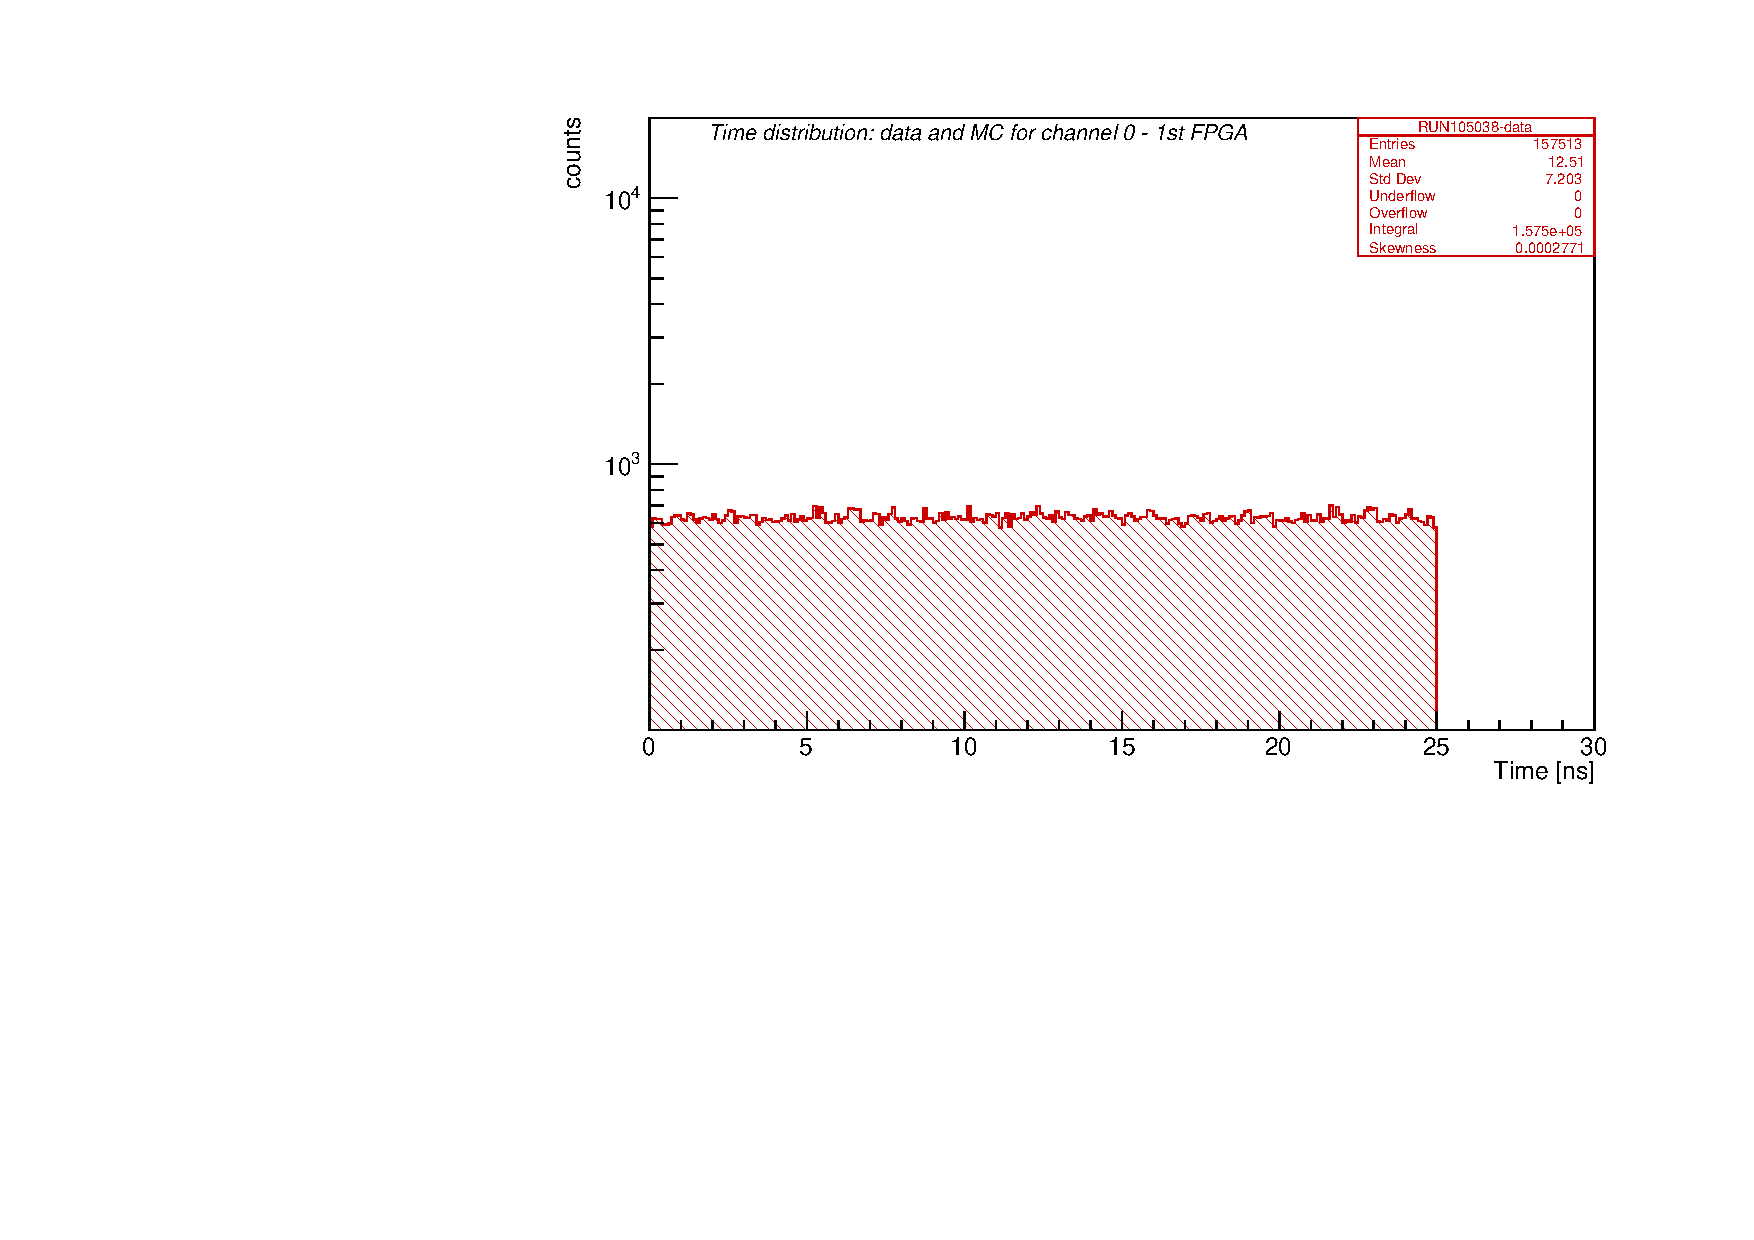
\includegraphics[width=0.5\textwidth]{figures/pdf/figure_00001_timedistr_roc_simulation_10538}
      % }
    };
    \node[anchor=south west,inner sep=0] at (10,0.) {
      % \node[shift={(0 cm,0.cm)},inner sep=0,rotate={90}] at (0,0) {}
      % \makebox[\textwidth][c] {
      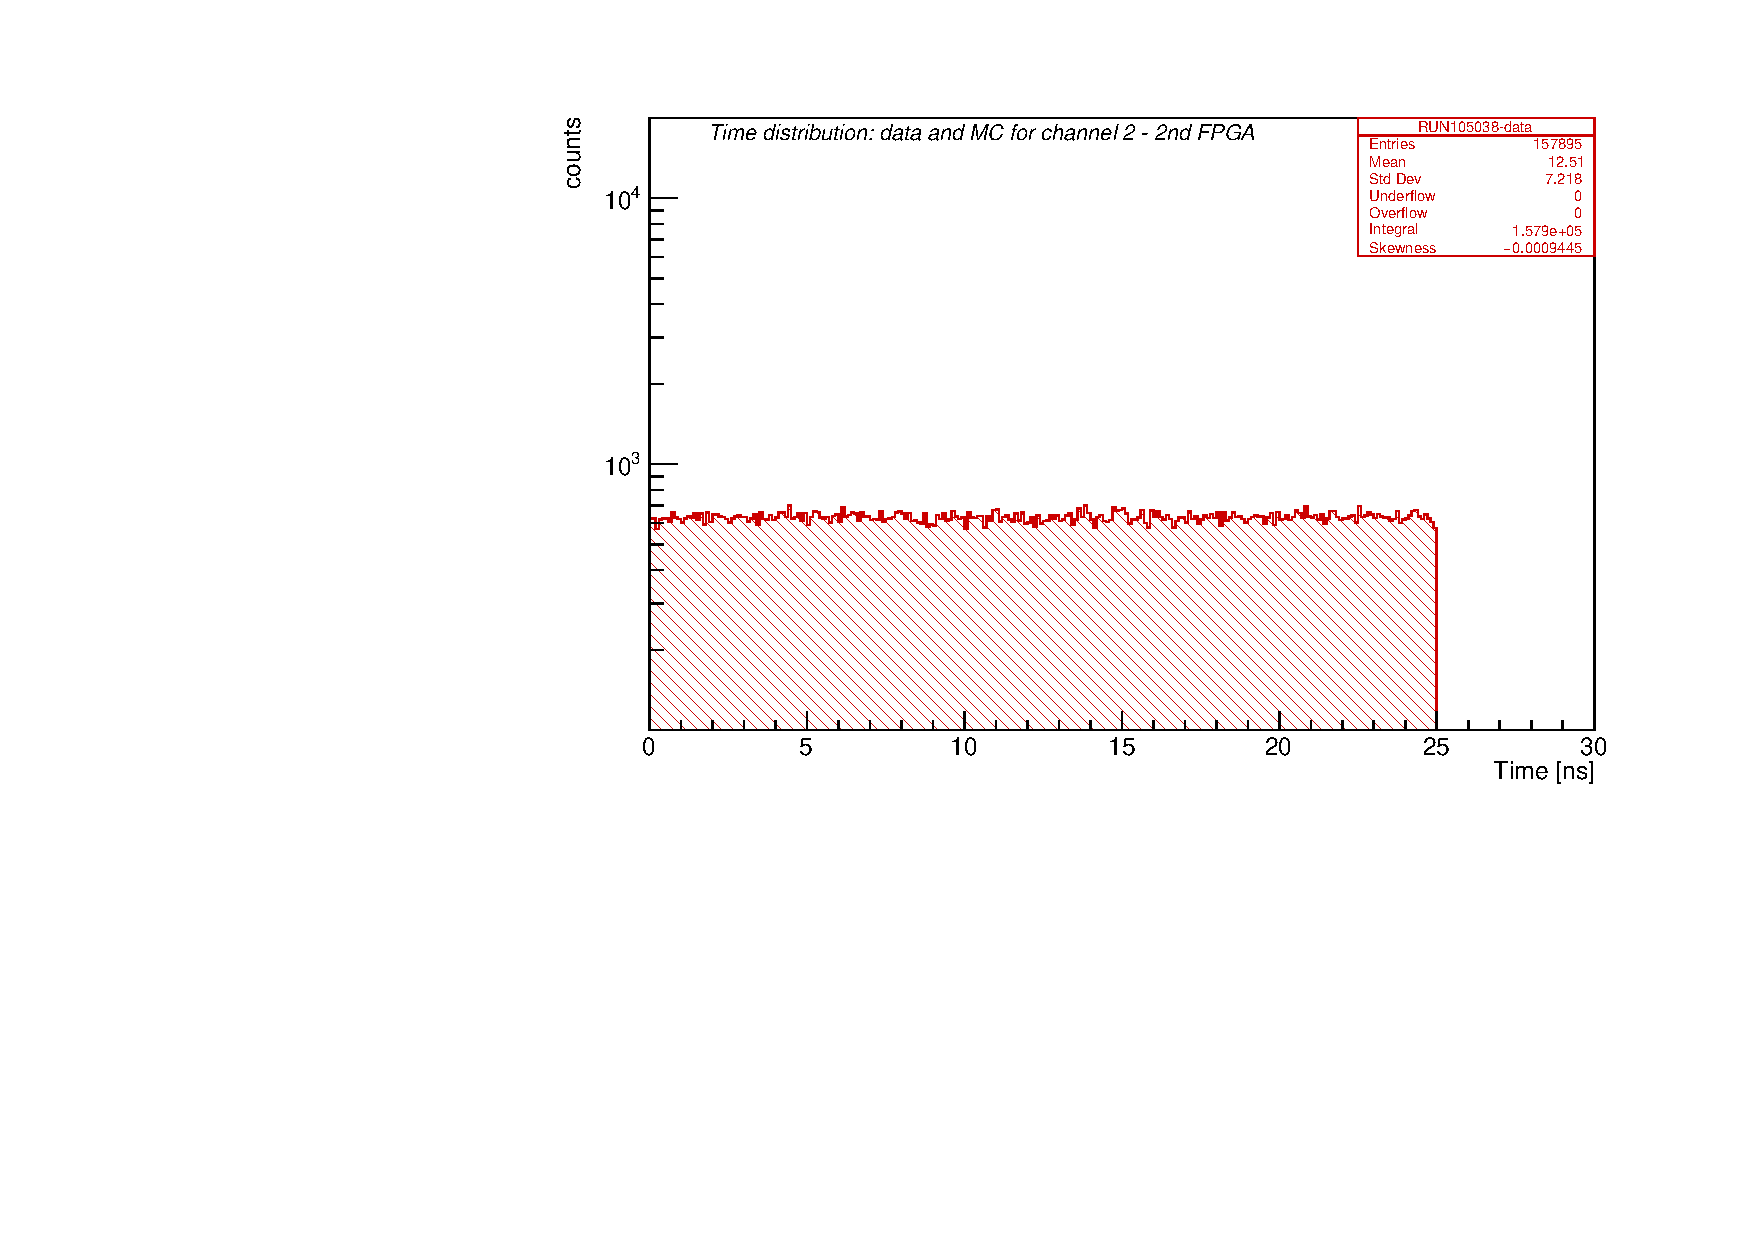
\includegraphics[width=0.5\textwidth]{figures/pdf/figure_00012_timedistr_roc_simulation_ch2_105038}
      % }
    };
  \end{tikzpicture}
  \caption{
    \label{fig:4}
    right: the hit time distribution for hits in channel 0, the first FPGA;
    left: the hit time distribution for this in channel 2, the second FPGA.
  }
\end{figure}
In this mode, the readout of a given channel is not affected by the readout of previous
channels and the ``occupancy'' distributions shown in Figure \ref{fig:5} are, as expected, uniform.
\begin{figure}[H]
\centering
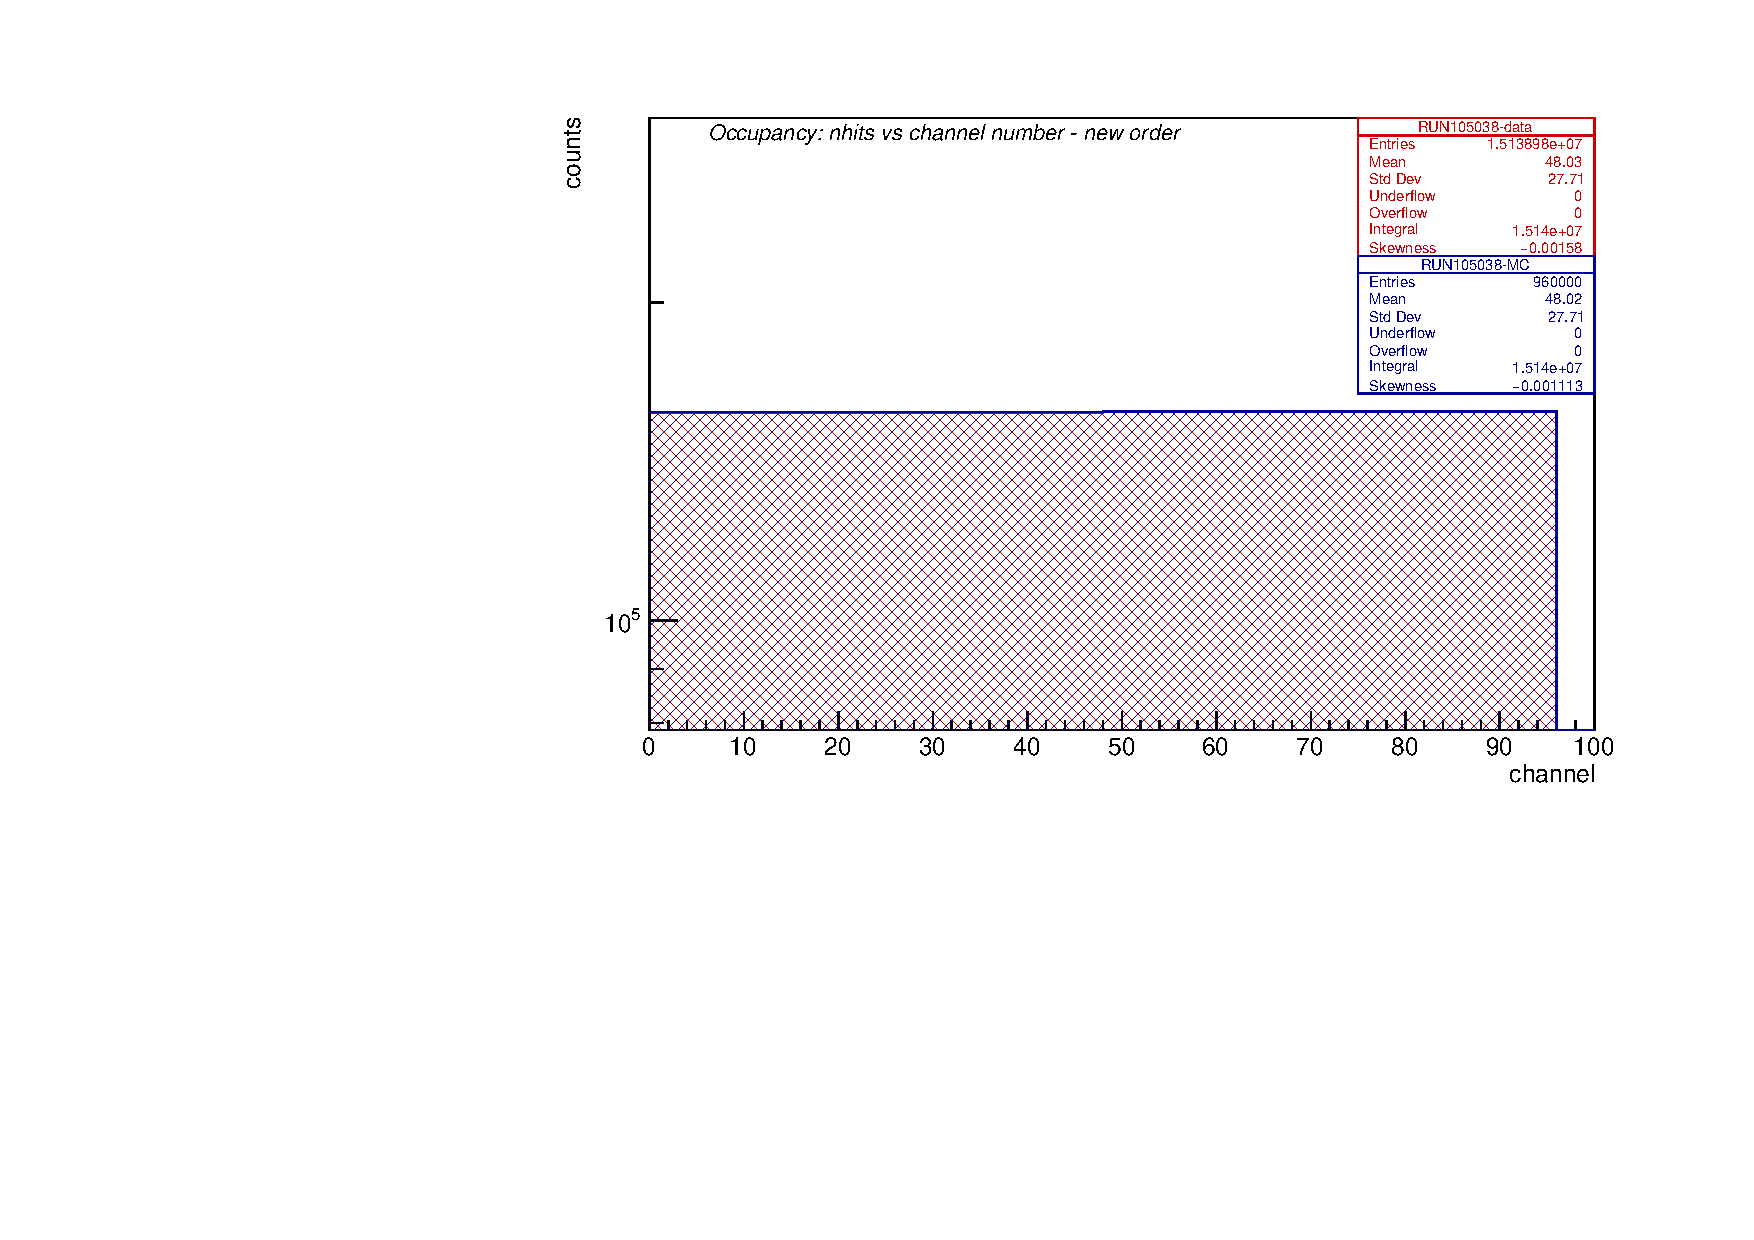
\includegraphics[width =0.8\textwidth]{figures/pdf/figure_00002_nhitsvschannel_roc_simulation_2}
\caption{Occupancy: the number of hits versus the channel number for run 105038.}
\label{fig:5}
\end{figure}


Fig.\ref{fig:67} shows the distribution of the number of hits in the channel 0 (first FPGA).
\begin{figure}[H]
\centering
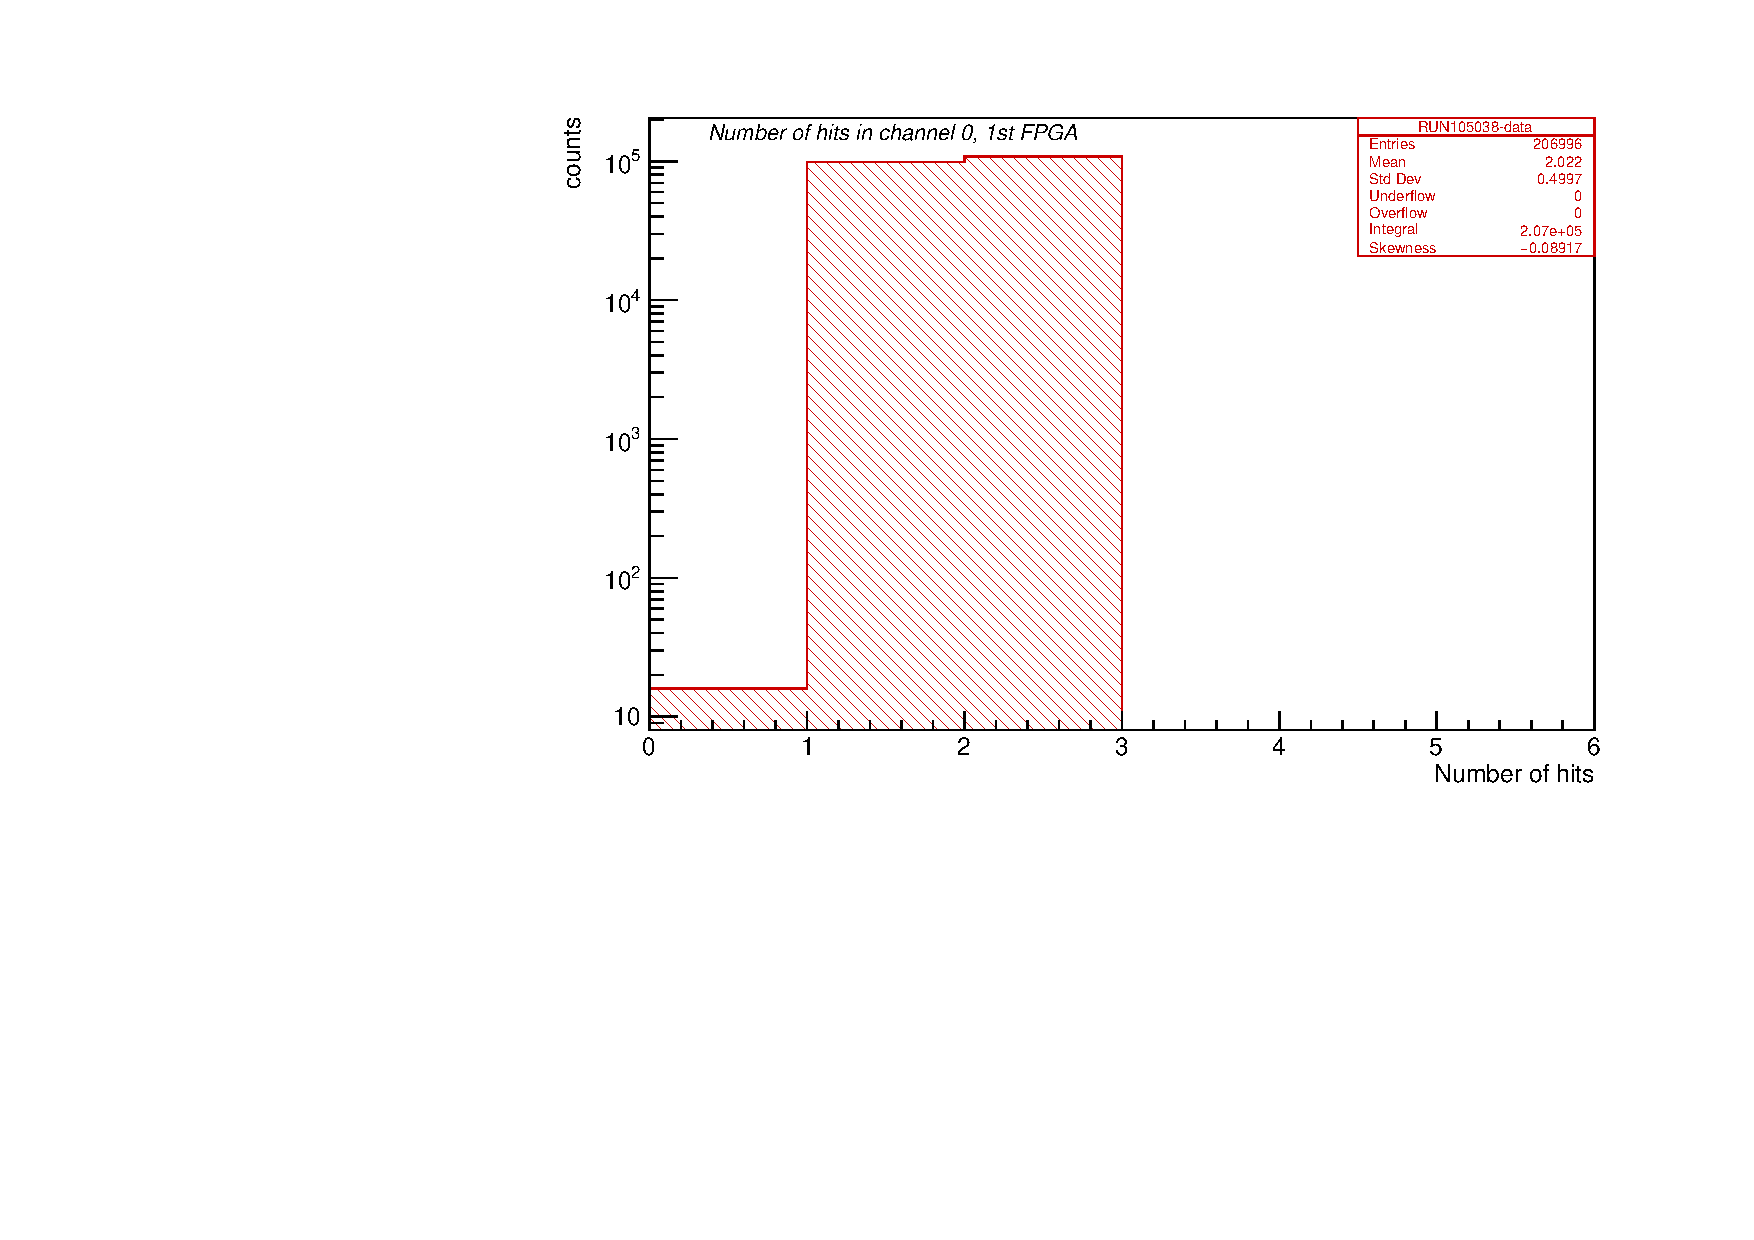
\includegraphics[width =0.8\textwidth]{figures/pdf/figure_00067_nhits_ch00_run105038.pdf}
\caption{
  The distribution of the number of hits in channel 0, first FPGA, for run 105038.
  Entries in the n(hits)=0 bin are due to the readout errors.
}
\label{fig:67}
\end{figure}

%%%%%%%%%%%%%%%%%%%%%%%%%%%%%%%%%%%%%%%%%%%%%%%%%%%%%%%%%%%%%%%%%%%%%%%%%%%%%%
\subsection{Number of hits}
Compared to run 281, the event window in run 105038 was x2 shorter
and the ROC readout buffer wasn't getting filled up.
The total number of hits within the event window depends on the relative offset
of the event window with respect to the FPGA pulsers, and varies from
144 to 192, as shown in Figure \ref{fig:6}.

\begin{figure}[!h]
\centering
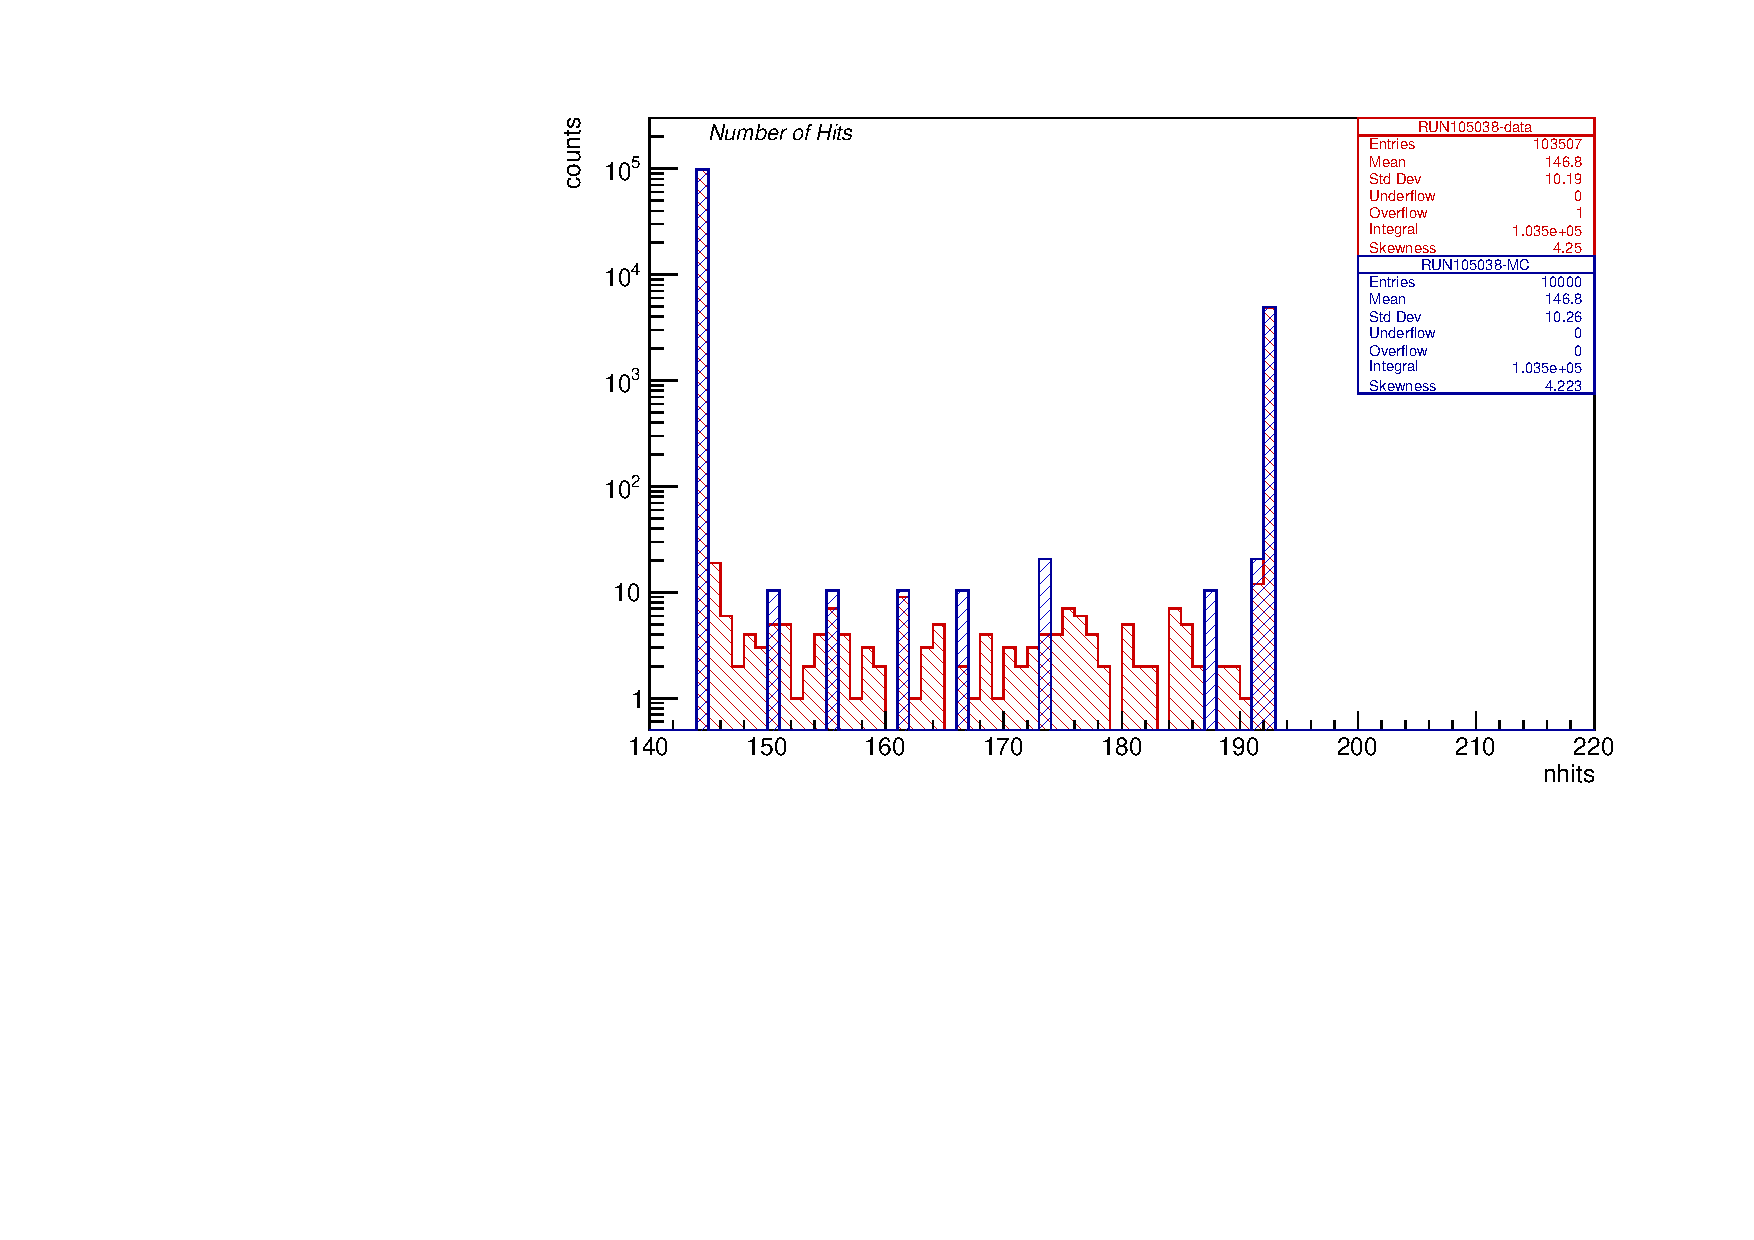
\includegraphics[width =0.8\textwidth]{figures/pdf/figure_00009_nhits_105038}
\caption{
  Distribution of the total number of hits per event in ``non-saturated'' mode
}
\label{fig:6}
\end{figure}










%%% Local Variables:
%%% mode: latex
%%% TeX-master: t
%%% End:
